\newline
Based on Table \vref{table:parameterSettings2} we see that the selected value for the parameter $s$ and $i$ are sat to respectively 150 and 100. However, one thing that is not considered in the initial parameter setting is that the size of $s$ and $i$ affects each other. A colony of 10 ants ran 100 times would produce similar results to 100 ants ran 10 times. Because of this additional tests are performed with respectively a colony size ($s$) of 50, 75, 100, 125 and 150 ran 100 iterations ($i$). The results of these tests are presented in Figure \vref{fig:svsitesting}.

\begin{figure}[H]
\begin{center}
  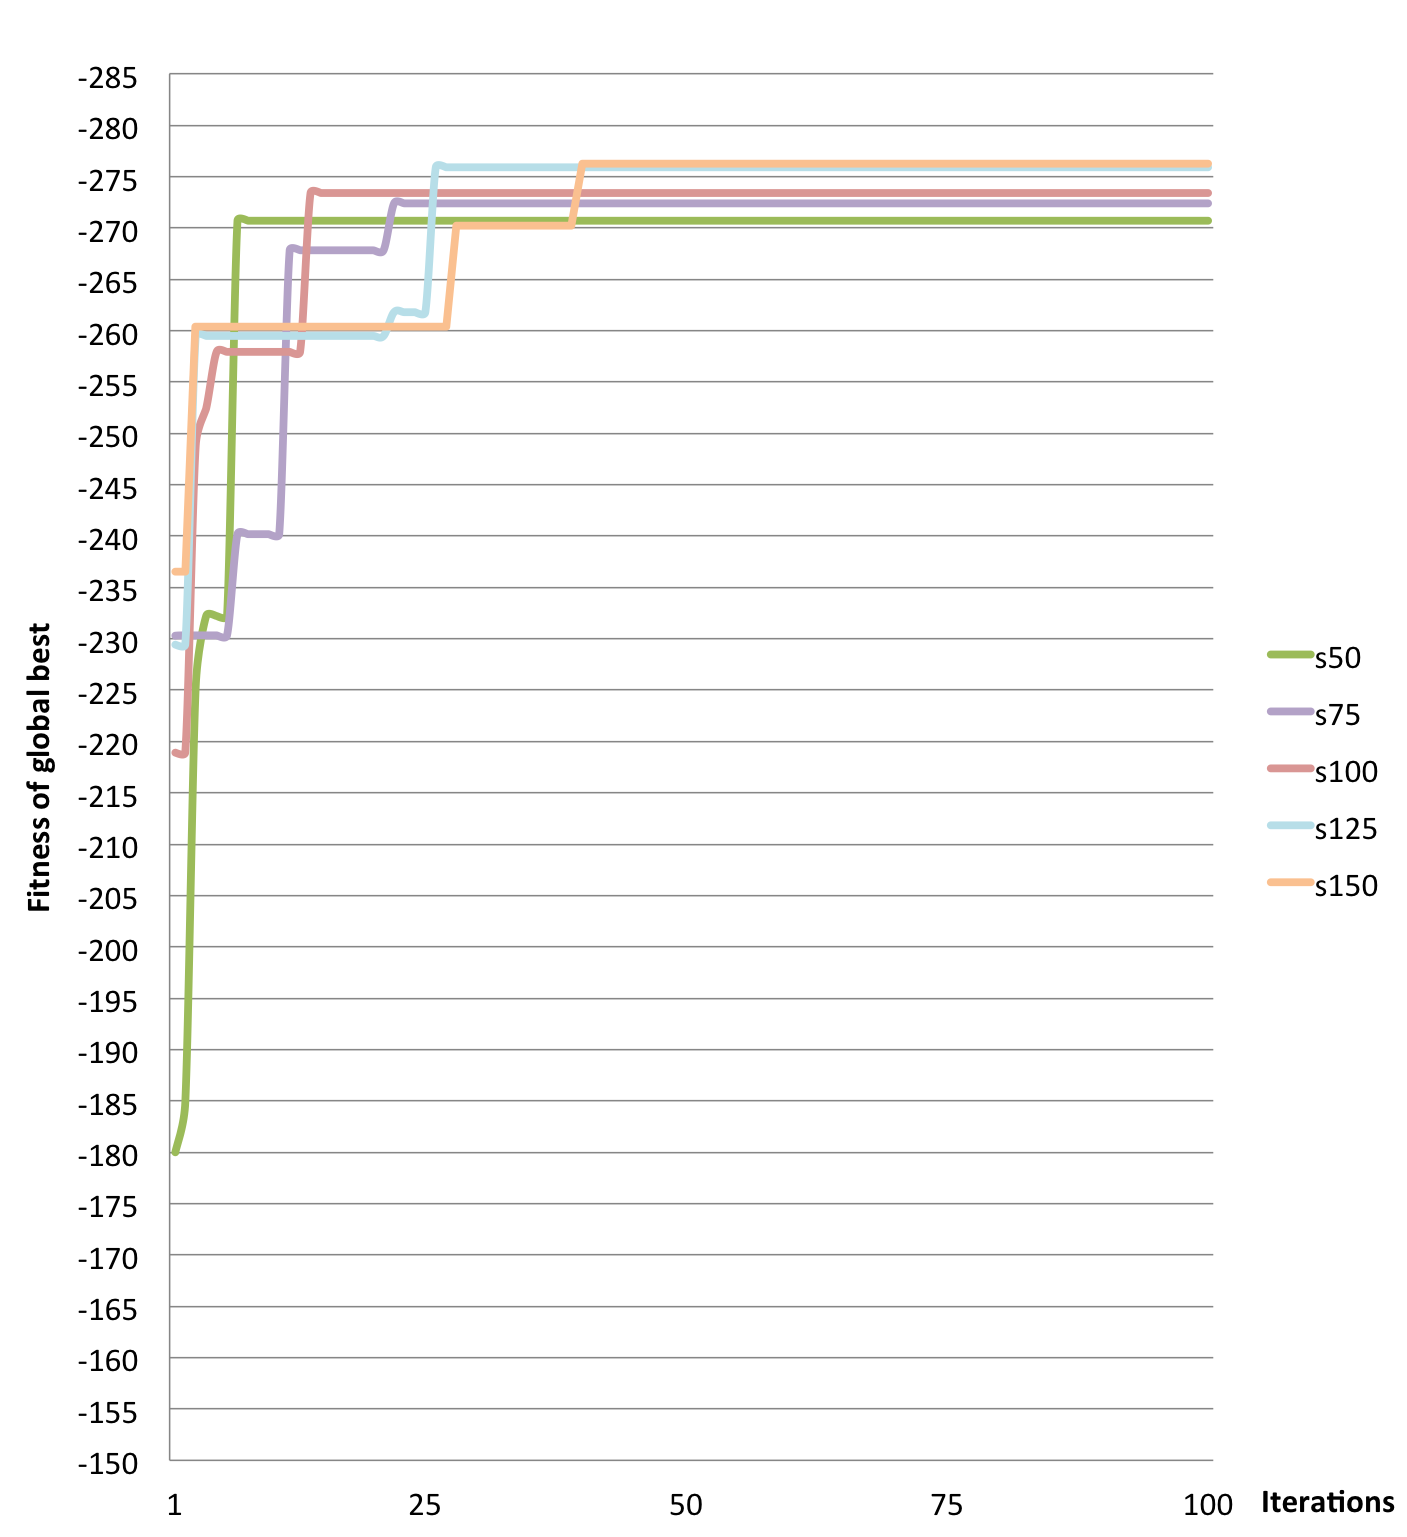
\includegraphics[width=4in]{assets/svsitest.png}
  \end{center}
  \caption{Evolution of total fitness function against the number of ants in the swarm (s)}
  \label{fig:svsitesting} 
\end{figure}

Figure \vref{fig:svsitesting} shows the evaluation of the total fitness ($TOTFIT$) of the global best ant with the colony sizes mentioned above. The algorithm is run one time for each swarm size, and the $TOTFIT$ value is recorded for each iteration. As one can see from Figure \vref{fig:svsitesting} increasing the size of the colony leads to a better $TOTFIT$ value in both the initial and final iterations.  %In the first iteration, all edge values are zero, and the first point in the graph represents the $TOTFIT$ value after the first iteration. 

However, there is a great difference in the running time when increasing the colony size. Figure \vref{fig:svsiruntime} presents the time it takes in seconds to run the algorithm one time with 100 iterations for each swarm size. As one can see there is a big difference in running time with 125 ants compared to 100. Between 50 and 100 ants the running time increases with about 750 seconds, while between 100 and 125 the running time increases with about 1200 seconds. 

\begin{figure}[H]
\begin{center}
  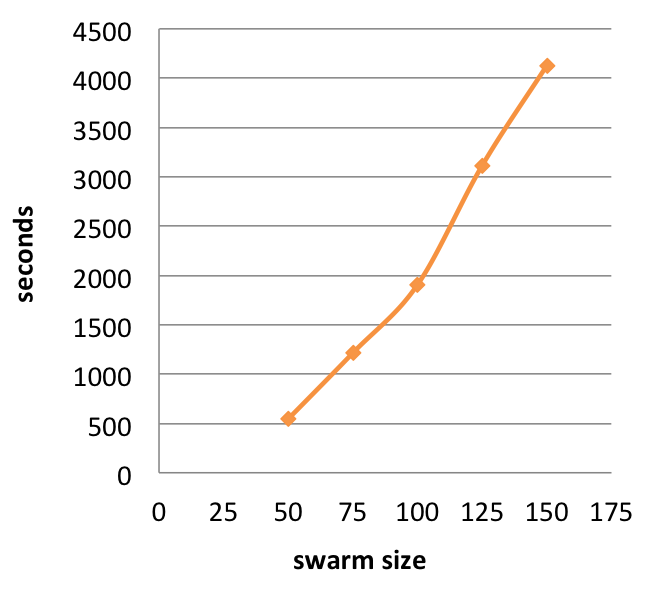
\includegraphics[width=2.5in]{assets/svsiruntime.png}
  \end{center}
  \caption{Evolution of the runtime, in seconds, in accordance to the swarm size}
  \label{fig:svsiruntime} 
\end{figure}

Because the algorithm is going to be run an excessive amount of times when testing performance comparison, the selected value of parameter $s$ is sat to \textit{100}. This is done, even though both a $s$ of both 125 and 150 gave a better $TOTFIT$, due to the large difference in run time. 

As one can see from Figure \vref{fig:svsitesting}, the algorithm seems to converge before 50 iterations, regardless of the colony size. This also corresponds to our initial parameter testing of $i$, which only shows a small improvement of the average $TOTFIT$ and the average travel time $ATT$ of 100 iterations compared to 50. The run time also increases drastically with 100 iterations compared to 50. The algorithm uses 499 seconds on the first 50 iterations, while it uses 1408 seconds on the last 50 iterations. These reasons combined makes the selected value of parameter $i$ \textit{50} and not 100, even tough 100 produced slightly better results in the initial parameter setting experiment.  

